\section{Referencia de la Clase Albaran\-Cliente\-View}
\label{classAlbaranClienteView}\index{AlbaranClienteView@{AlbaranClienteView}}
Muestra el albar\'{a}n a cliente.  


{\tt \#include $<$albaranclienteview.h$>$}

Diagrama de herencias de Albaran\-Cliente\-View\begin{figure}[H]
\begin{center}
\leavevmode
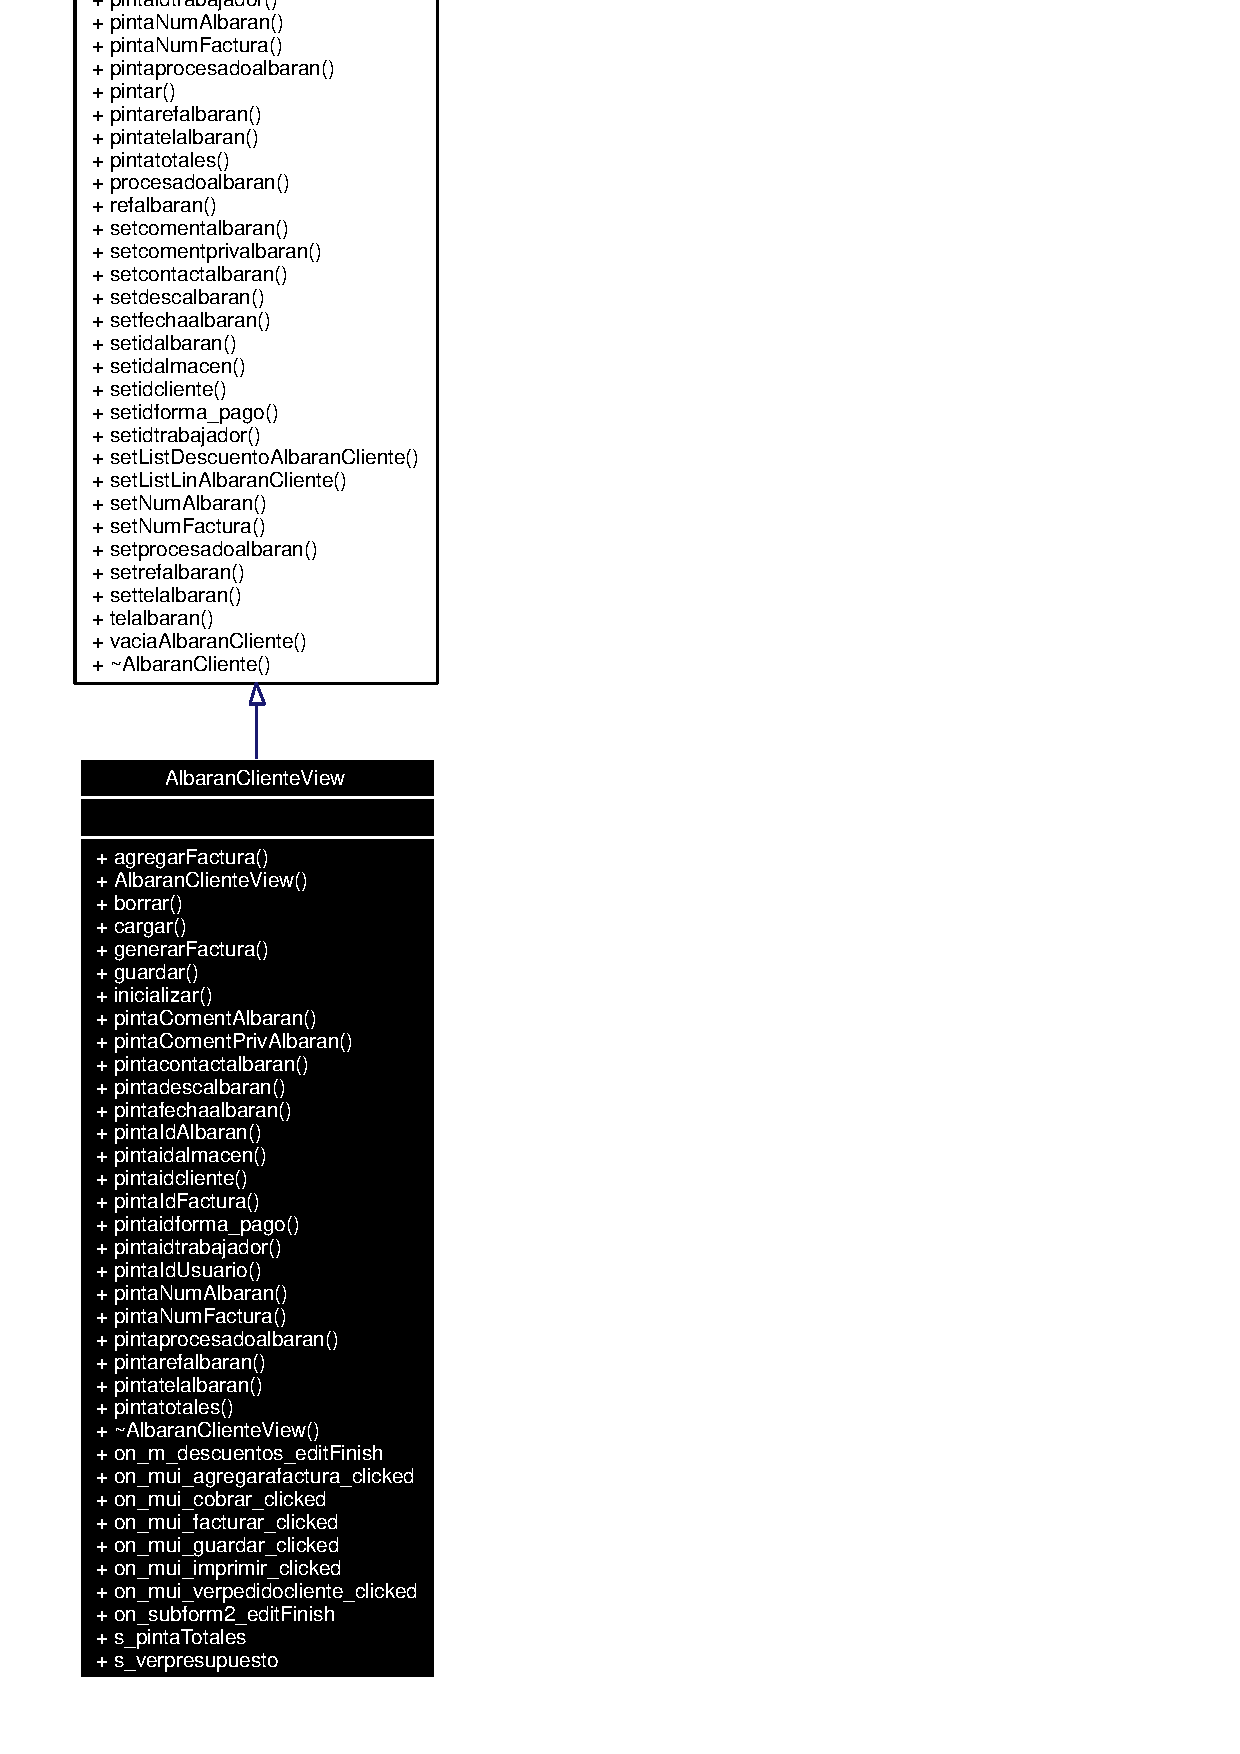
\includegraphics[width=105pt]{classAlbaranClienteView__inherit__graph}
\end{center}
\end{figure}
Diagrama de colaboraci\'{o}n para Albaran\-Cliente\-View:\begin{figure}[H]
\begin{center}
\leavevmode
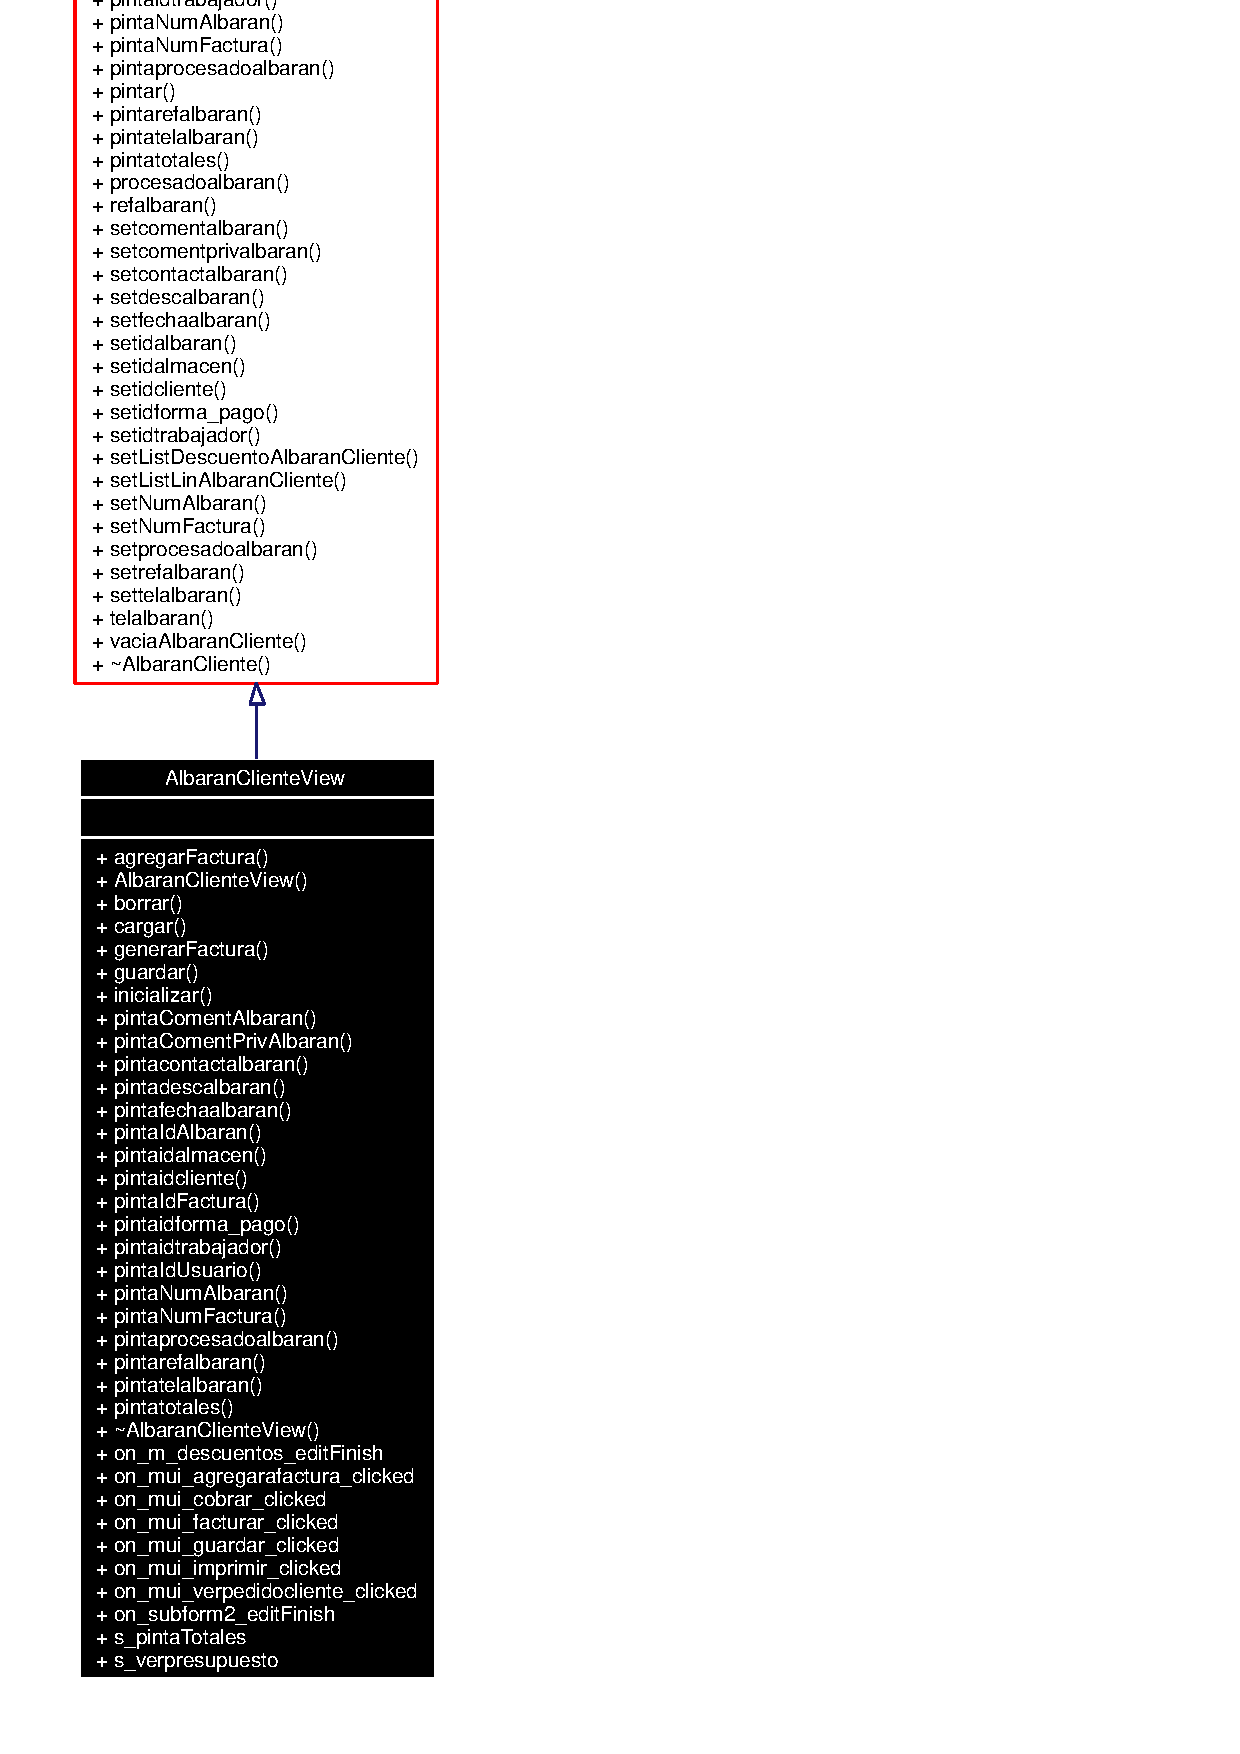
\includegraphics[width=105pt]{classAlbaranClienteView__coll__graph}
\end{center}
\end{figure}
\subsection*{Slots p\'{u}blicos}
\begin{CompactItemize}
\item 
virtual void {\bf on\_\-m\_\-descuentos\_\-edit\-Finish} (int, int)\label{classAlbaranClienteView_i0}

\item 
virtual void {\bf on\_\-mui\_\-agregarafactura\_\-clicked} ()\label{classAlbaranClienteView_i1}

\item 
virtual void {\bf on\_\-mui\_\-cobrar\_\-clicked} ()\label{classAlbaranClienteView_i2}

\begin{CompactList}\small\item\em Crea un nuevo cobro para el albar\'{a}n seleccionado. \item\end{CompactList}\item 
virtual void {\bf on\_\-mui\_\-facturar\_\-clicked} ()\label{classAlbaranClienteView_i3}

\item 
virtual void {\bf on\_\-mui\_\-guardar\_\-clicked} ()\label{classAlbaranClienteView_i4}

\item 
virtual void {\bf on\_\-mui\_\-imprimir\_\-clicked} ()\label{classAlbaranClienteView_i5}

\item 
virtual void {\bf on\_\-mui\_\-verpedidocliente\_\-clicked} ()\label{classAlbaranClienteView_i6}

\item 
virtual void {\bf on\_\-subform2\_\-edit\-Finish} (int, int)\label{classAlbaranClienteView_i7}

\item 
virtual void {\bf s\_\-pinta\-Totales} ()\label{classAlbaranClienteView_i8}

\begin{CompactList}\small\item\em Este slot se activa cuando hay cambios en los subformularios. \item\end{CompactList}\item 
virtual void {\bf s\_\-verpresupuesto} ()\label{classAlbaranClienteView_i9}

\end{CompactItemize}
\subsection*{M\'{e}todos p\'{u}blicos}
\begin{CompactItemize}
\item 
void {\bf agregar\-Factura} ()
\begin{CompactList}\small\item\em Se encarga de agregar un albaran a una factura. \item\end{CompactList}\item 
{\bf Albaran\-Cliente\-View} ({\bf company} $\ast$, QWidget $\ast$)\label{classAlbaranClienteView_a1}

\item 
virtual int {\bf borrar} ()\label{classAlbaranClienteView_a2}

\item 
virtual int {\bf cargar} (QString id)\label{classAlbaranClienteView_a3}

\begin{CompactList}\small\item\em Esta funcioncarga un {\bf Albaran\-Cliente}{\rm (p.\,\pageref{classAlbaranCliente})}. \item\end{CompactList}\item 
void {\bf generar\-Factura} ()
\begin{CompactList}\small\item\em Se encarga de generar una factura a partir de un albar\'{a}n. \item\end{CompactList}\item 
virtual int {\bf guardar} ()
\begin{CompactList}\small\item\em Estos metodos deben existir para poder trabajar con la clase Ficha. \item\end{CompactList}\item 
void {\bf inicializar} ()\label{classAlbaranClienteView_a6}

\item 
void {\bf pinta\-Coment\-Albaran} (QString val)\label{classAlbaranClienteView_a7}

\item 
void {\bf pinta\-Coment\-Priv\-Albaran} (QString val)\label{classAlbaranClienteView_a8}

\item 
void {\bf pintacontactalbaran} (QString val)\label{classAlbaranClienteView_a9}

\item 
void {\bf pintadescalbaran} (QString val)\label{classAlbaranClienteView_a10}

\item 
void {\bf pintafechaalbaran} (QString val)\label{classAlbaranClienteView_a11}

\item 
void {\bf pinta\-Id\-Albaran} (QString)\label{classAlbaranClienteView_a12}

\item 
void {\bf pintaidalmacen} (QString id)\label{classAlbaranClienteView_a13}

\item 
void {\bf pintaidcliente} (QString val)\label{classAlbaranClienteView_a14}

\item 
void {\bf pinta\-Id\-Factura} (QString)\label{classAlbaranClienteView_a15}

\item 
void {\bf pintaidforma\_\-pago} (QString val)\label{classAlbaranClienteView_a16}

\item 
void {\bf pintaidtrabajador} (QString id)\label{classAlbaranClienteView_a17}

\item 
void {\bf pinta\-Id\-Usuario} (QString)\label{classAlbaranClienteView_a18}

\item 
void {\bf pinta\-Num\-Albaran} (QString val)\label{classAlbaranClienteView_a19}

\item 
void {\bf pinta\-Num\-Factura} (QString)\label{classAlbaranClienteView_a20}

\item 
void {\bf pintaprocesadoalbaran} (QString id)\label{classAlbaranClienteView_a21}

\item 
void {\bf pintarefalbaran} (QString val)\label{classAlbaranClienteView_a22}

\item 
void {\bf pintatelalbaran} (QString val)\label{classAlbaranClienteView_a23}

\item 
void {\bf pintatotales} (Fixed, Fixed, Fixed, Fixed)\label{classAlbaranClienteView_a24}

\end{CompactItemize}


\subsection{Descripci\'{o}n detallada}
Muestra el albar\'{a}n a cliente. 



\subsection{Documentaci\'{o}n de las funciones miembro}
\index{AlbaranClienteView@{Albaran\-Cliente\-View}!agregarFactura@{agregarFactura}}
\index{agregarFactura@{agregarFactura}!AlbaranClienteView@{Albaran\-Cliente\-View}}
\subsubsection{\setlength{\rightskip}{0pt plus 5cm}void Albaran\-Cliente\-View::agregar\-Factura ()}\label{classAlbaranClienteView_a0}


Se encarga de agregar un albaran a una factura. 

Pedimos la factura a la que agregar.

Hacemos que las opciones de filtrado del listado ya est\'{e}n bien.

Lanzamos el di\'{a}logo.

Si no hay idfactura es que hemos abortado y por tanto cancelamos la operaci\'{o}n.

Creamos la factura.

Agregamos en los comentarios que se ha a\~{n}adido este albar\'{a}n.

EN TEORIA SE DEBARIA COMPROBAR QUE LA FACTURA ES DEL MISMO CLIENTE, pero por ahora pasamos de hacerlo. \index{AlbaranClienteView@{Albaran\-Cliente\-View}!generarFactura@{generarFactura}}
\index{generarFactura@{generarFactura}!AlbaranClienteView@{Albaran\-Cliente\-View}}
\subsubsection{\setlength{\rightskip}{0pt plus 5cm}void Albaran\-Cliente\-View::generar\-Factura ()}\label{classAlbaranClienteView_a4}


Se encarga de generar una factura a partir de un albar\'{a}n. 

Comprobamos que existe el elemento, y en caso afirmativo lo mostramos y salimos de la funci\'{o}n.

Informamos de que no existe el pedido y a ver si lo queremos realizar. Si no salimos de la funci\'{o}n.

Creamos la factura.

Cargamos un elemento que no existe para inicializar bien la clase. \index{AlbaranClienteView@{Albaran\-Cliente\-View}!guardar@{guardar}}
\index{guardar@{guardar}!AlbaranClienteView@{Albaran\-Cliente\-View}}
\subsubsection{\setlength{\rightskip}{0pt plus 5cm}int Albaran\-Cliente\-View::guardar ()\hspace{0.3cm}{\tt  [virtual]}}\label{classAlbaranClienteView_a5}


Estos metodos deben existir para poder trabajar con la clase Ficha. 

Cogemos todos los valores del formulario y actualizamos la clase.

Hacemos el guardado. 

Reimplementado de {\bf Albaran\-Cliente} {\rm (p.\,\pageref{classAlbaranCliente_a11})}.

La documentaci\'{o}n para esta clase fu\'{e} generada a partir de los siguientes archivos:\begin{CompactItemize}
\item 
albaranclienteview.h\item 
albaranclienteview.cpp\end{CompactItemize}
